

On analyse dans cette section, le prix du $CALL$ ou du $PUT$ à l'aide du modèle binomial. La Figure~\ref{fig:arbre} nous donne un reprèsentation simplifiée du modèle, qui aide à comprendre l'implémentation des algorithmes réalisés. 
La fonction permettant de calculer ces valeurs est Listing~\ref{listing:3}, elle est implémentée dans le fichier \textsc{arbre.py}.

\emph{Note: Dans le fichier code \textsc{arbre.py}, on a laissé plusieurs implémentations pour réaliser de mêmes calculs. La raison de ce choix est que certaines implémentations, n'étaient pas assez efficientes et causaient un \textbf{Stackoverflow}. On les a marqué comme \textbf{"optionelles"}}.

\begin{figure}[H]
\centering
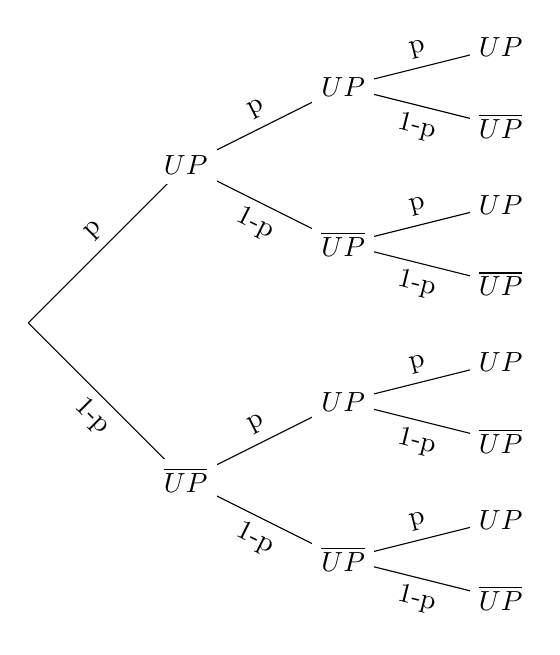
\begin{tikzpicture}[xscale=1,yscale=1]
\draw (0,0)--(-2,0.5) node[midway, below, sloped]{1-p};
\draw (0,1)--(-2,0.5) node[midway, above, sloped]{p};
\draw (0,2)--(-2,2.5) node[midway, below, sloped]{1-p};
\draw (0,3)--(-2,2.5) node[midway, above, sloped]{p};
\draw (0,4)--(-2,4.5) node[midway, below, sloped]{1-p};
\draw (0,5)--(-2,4.5) node[midway, above, sloped]{p};
\draw (0,6)--(-2,6.5) node[midway, below, sloped]{1-p};
\draw (0,7)--(-2,6.5) node[midway, above, sloped]{p};
\draw (-2,0.5)--(-4,1.5) node[midway, below, sloped]{1-p};
\draw (-2,2.5)--(-4,1.5) node[midway, above, sloped]{p};
\draw (-2,4.5)--(-4,5.5) node[midway, below, sloped]{1-p};
\draw (-2,6.5)--(-4,5.5) node[midway, above, sloped]{p};
\draw (-4,1.5)--(-6,3.5) node[midway, below, sloped]{1-p};
\draw (-4,5.5)--(-6,3.5) node[midway, above, sloped]{p};
\draw (0,0) node[fill=white]{$\overline{UP}$};
\draw (0,1) node[fill=white]{$UP$};
\draw (0,2) node[fill=white]{$\overline{UP}$};
\draw (0,3) node[fill=white]{$UP$};
\draw (0,4) node[fill=white]{$\overline{UP}$};
\draw (0,5) node[fill=white]{$UP$};
\draw (0,6) node[fill=white]{$\overline{UP}$};
\draw (0,7) node[fill=white]{$UP$};
\draw (-2,0.5) node[fill=white]{$\overline{UP}$};
\draw (-2,2.5) node[fill=white]{$UP$};
\draw (-2,4.5) node[fill=white]{$\overline{UP}$};
\draw (-2,6.5) node[fill=white]{$UP$};
\draw (-4,1.5) node[fill=white]{$\overline{UP}$};
\draw (-4,5.5) node[fill=white]{$UP$};
\end{tikzpicture}
\caption{Variation du prix du CALL en fonction date d'échéance T}
\label{fig:arbre}
\end{figure}

\subsection{Prix du $CALL$ ou du $PUT$ avec 20 pas} % (fold)
\label{sub:prix_du_call_ou_du_put_avec_20_pas}

\begin{table}[H]
	\centering
\begin{tabular}{|c|c|}
\hline
Option & Prix de l'option\\
\hline
CALL européen & 5.37\\
\hline
CALL américain & 5.37\\
\hline
PUT européen & 4.63\\
\hline
PUT américain & 4.70\\
\hline 
\end{tabular}
\caption{Prix des différentes options calculées par récurrence avec le modèle binomial}
\label{tab:prix-20}
\end{table}
% subsection prix_du_call_ou_du_put_avec_20_pas (end)

\subsection{Analyse de la variation du prix de l'option en fonction du nombre de pas} % (fold)
\label{sub:analyse_de_la_variation_du_prix_de_l_option_en_fonction_du_nombre_de_pas}

% subsection analyse_de_la_variation_du_prix_de_l_option_en_fonction_du_nombre_de_pas (end)
On observe sur la Figure~\ref{fig:call_euro_mb} et Figure~\ref{fig:put_euro_mb}, que le prix des options européennes tendent vers le prix obtenus avec le modèle de Black et Scholes. Ce résultat était prévisible, de part la \textbf{construction} du modèle de Black et Scholes :
$$\lim_{pas\rightarrow \infty} PRIX(CALL)_{BINOM}=PRIX(CALL)_{BLACK ET SCHOLES}$$

Pour ce qui est des options américaines on observe sur la Figure~\ref{fig:call_amer_mb}, et Figure~\ref{fig:put_amer_mb} que $CALL_{amer}=CALL_{euro}$ et $PUT_{amer}\geq PUT_{euro}$. Ce qui est cohérent avec le \textbf{principe de non-domination} (AOA). En effet on a d'après la parité $CALL, PUT$ et le \textbf{principe de non-domination} (AOA): 
\[
	 CALL_T(T,K)-PUT_T(T,K)=S_T-K 
\]
\[
	\Leftrightarrow CALL_t(T,K)-PUT_t(T,K)=S_t-KB_t(T)  \ \text{(AOA)}
\]

On obtiens donc les bornes suivantes : 
\[
	(S_t-K)^+ \leq CALL_t(T,K) \leq S_t \qquad (KB_t(T)-S_t)^+ \leq PUT_t(T,K) \leq KB_t(T)
\]

De plus il est évident que $CALL_{amer}\geq CALL_{euro}$ et $PUT_{amer}\geq PUT_{euro}$ puisqu'elles peuvent être éxecutées à tout moment, ce qui explique Figure~\ref{fig:put_amer_mb}. Cependant d'après les bornes antérieures on a : 
\[
	CALL_{amer}\geq CALL_{euro}> (S_t-K)^+ \quad \forall t < T
\]
Il n'est donc jamais optimal d'exercer le call américain avant échéance (s'il n'y a pas de dividendes), d'où l'égalité observée sur Figure~\ref{fig:call_euro_mb}.

\begin{figure}[H]
\centering
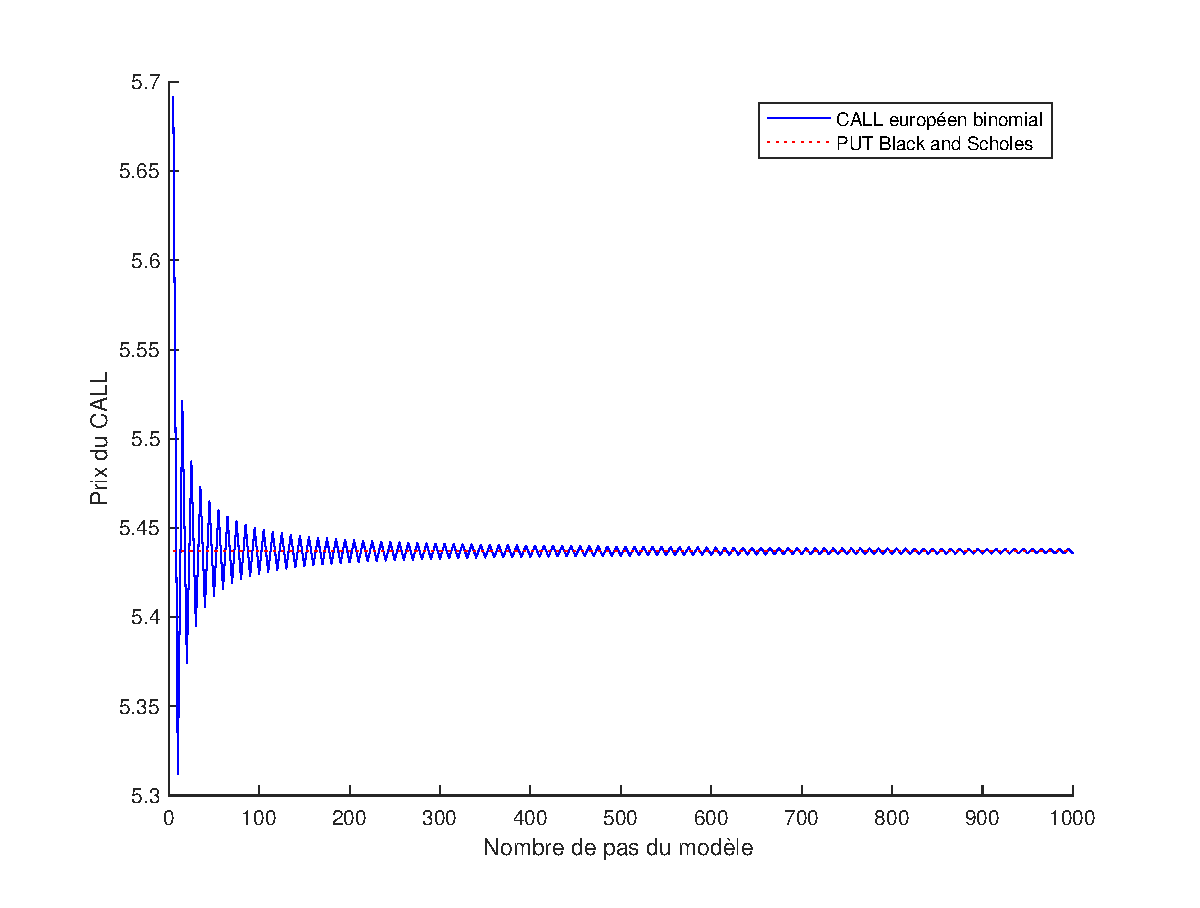
\includegraphics[scale=0.6]{./img/CALL_EURO-BS.eps}
\caption{Variation du prix du CALL européen en fonction du nombre de pas}
\label{fig:call_euro_mb}
\end{figure}

\begin{figure}[H]
\centering
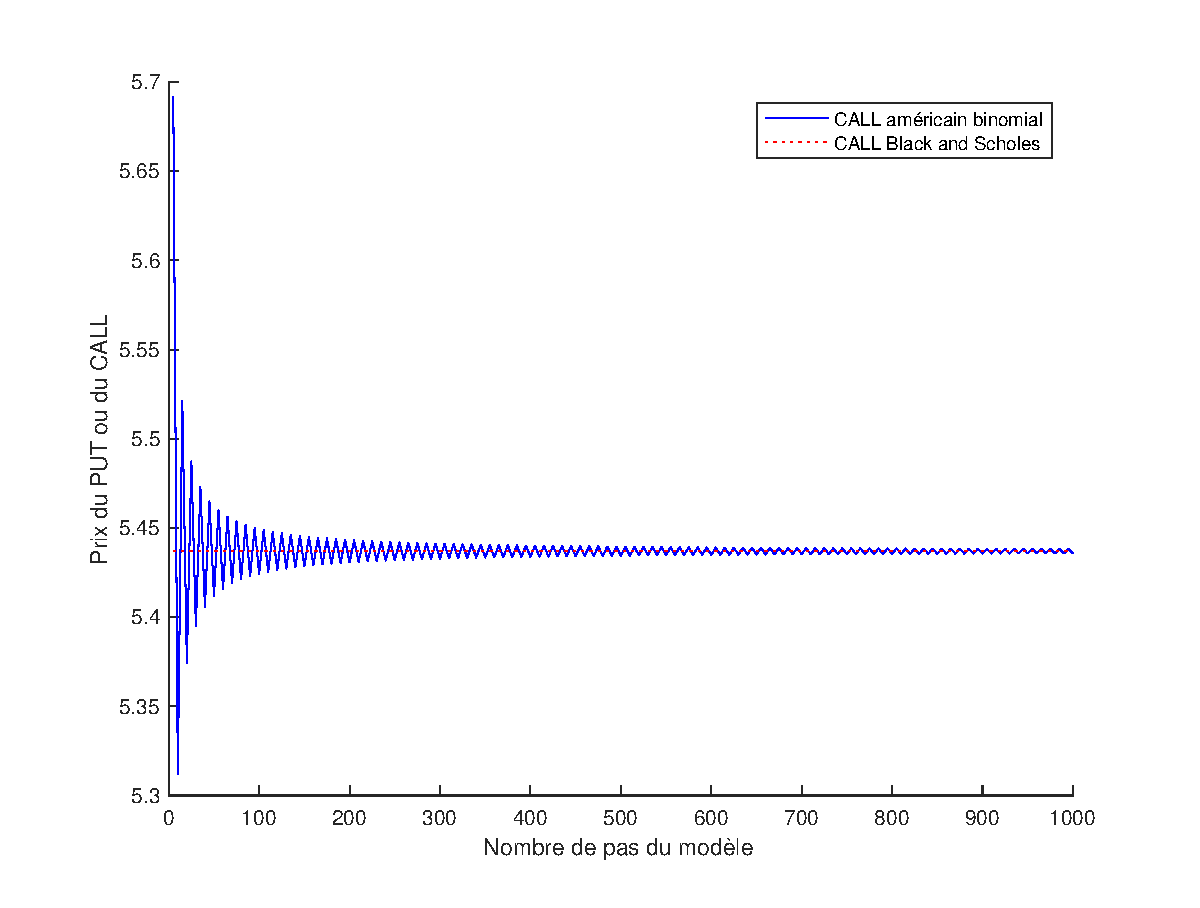
\includegraphics[scale=0.6]{./img/CALL_AMER-BS.eps}
\caption{Variation du prix du CALL européen en fonction du nombre de pas}
\label{fig:call_amer_mb}
\end{figure}

\begin{figure}[H]
\centering
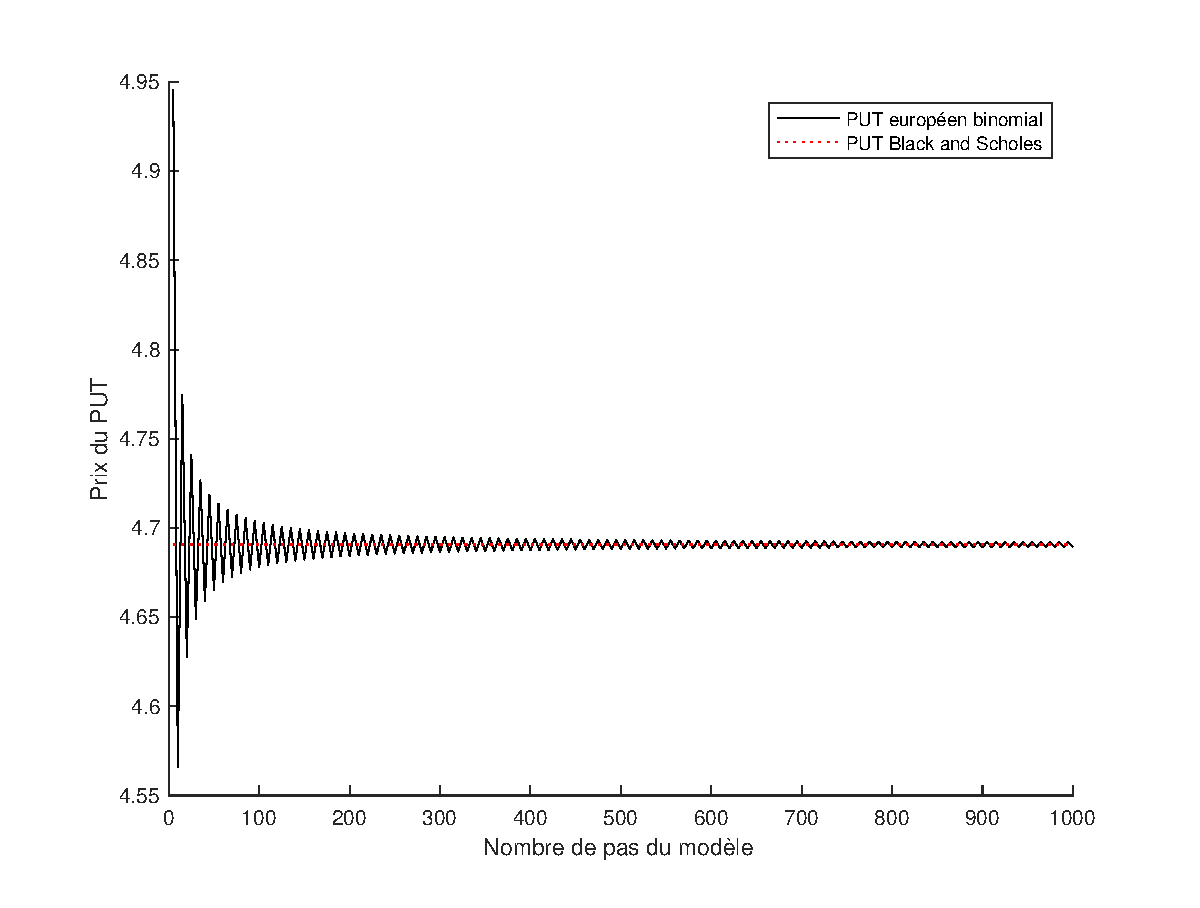
\includegraphics[scale=0.6]{./img/PUT_EURO-BS.eps}
\caption{Variation du prix du PUT européen en fonction du nombre de pas}
\label{fig:put_euro_mb}
\end{figure}

\begin{figure}[H]
\centering
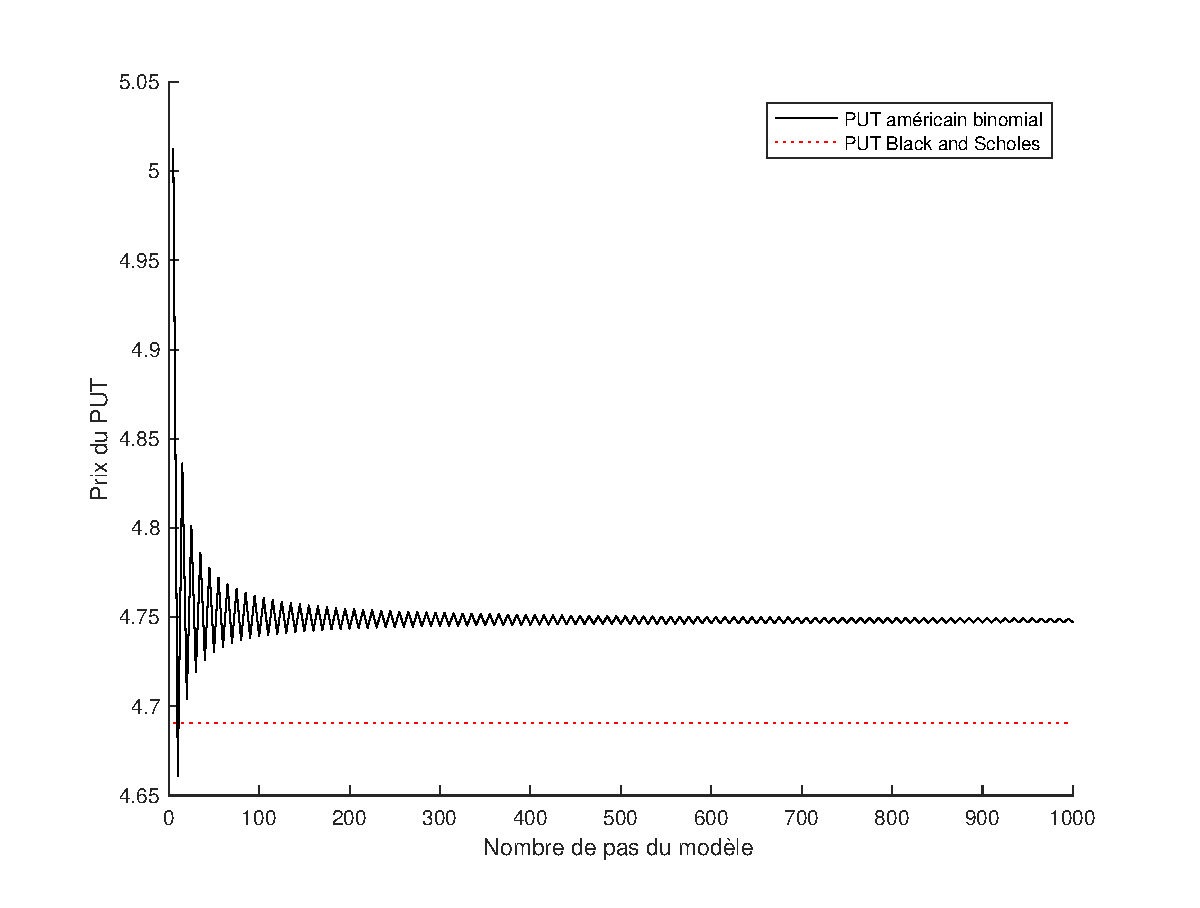
\includegraphics[scale=0.6]{./img/PUT_AMER-BS.eps}
\caption{Variation du prix du PUT américain en fonction du nombre de pas}
\label{fig:put_amer_mb}
\end{figure}

\begin{figure}[H]
\centering
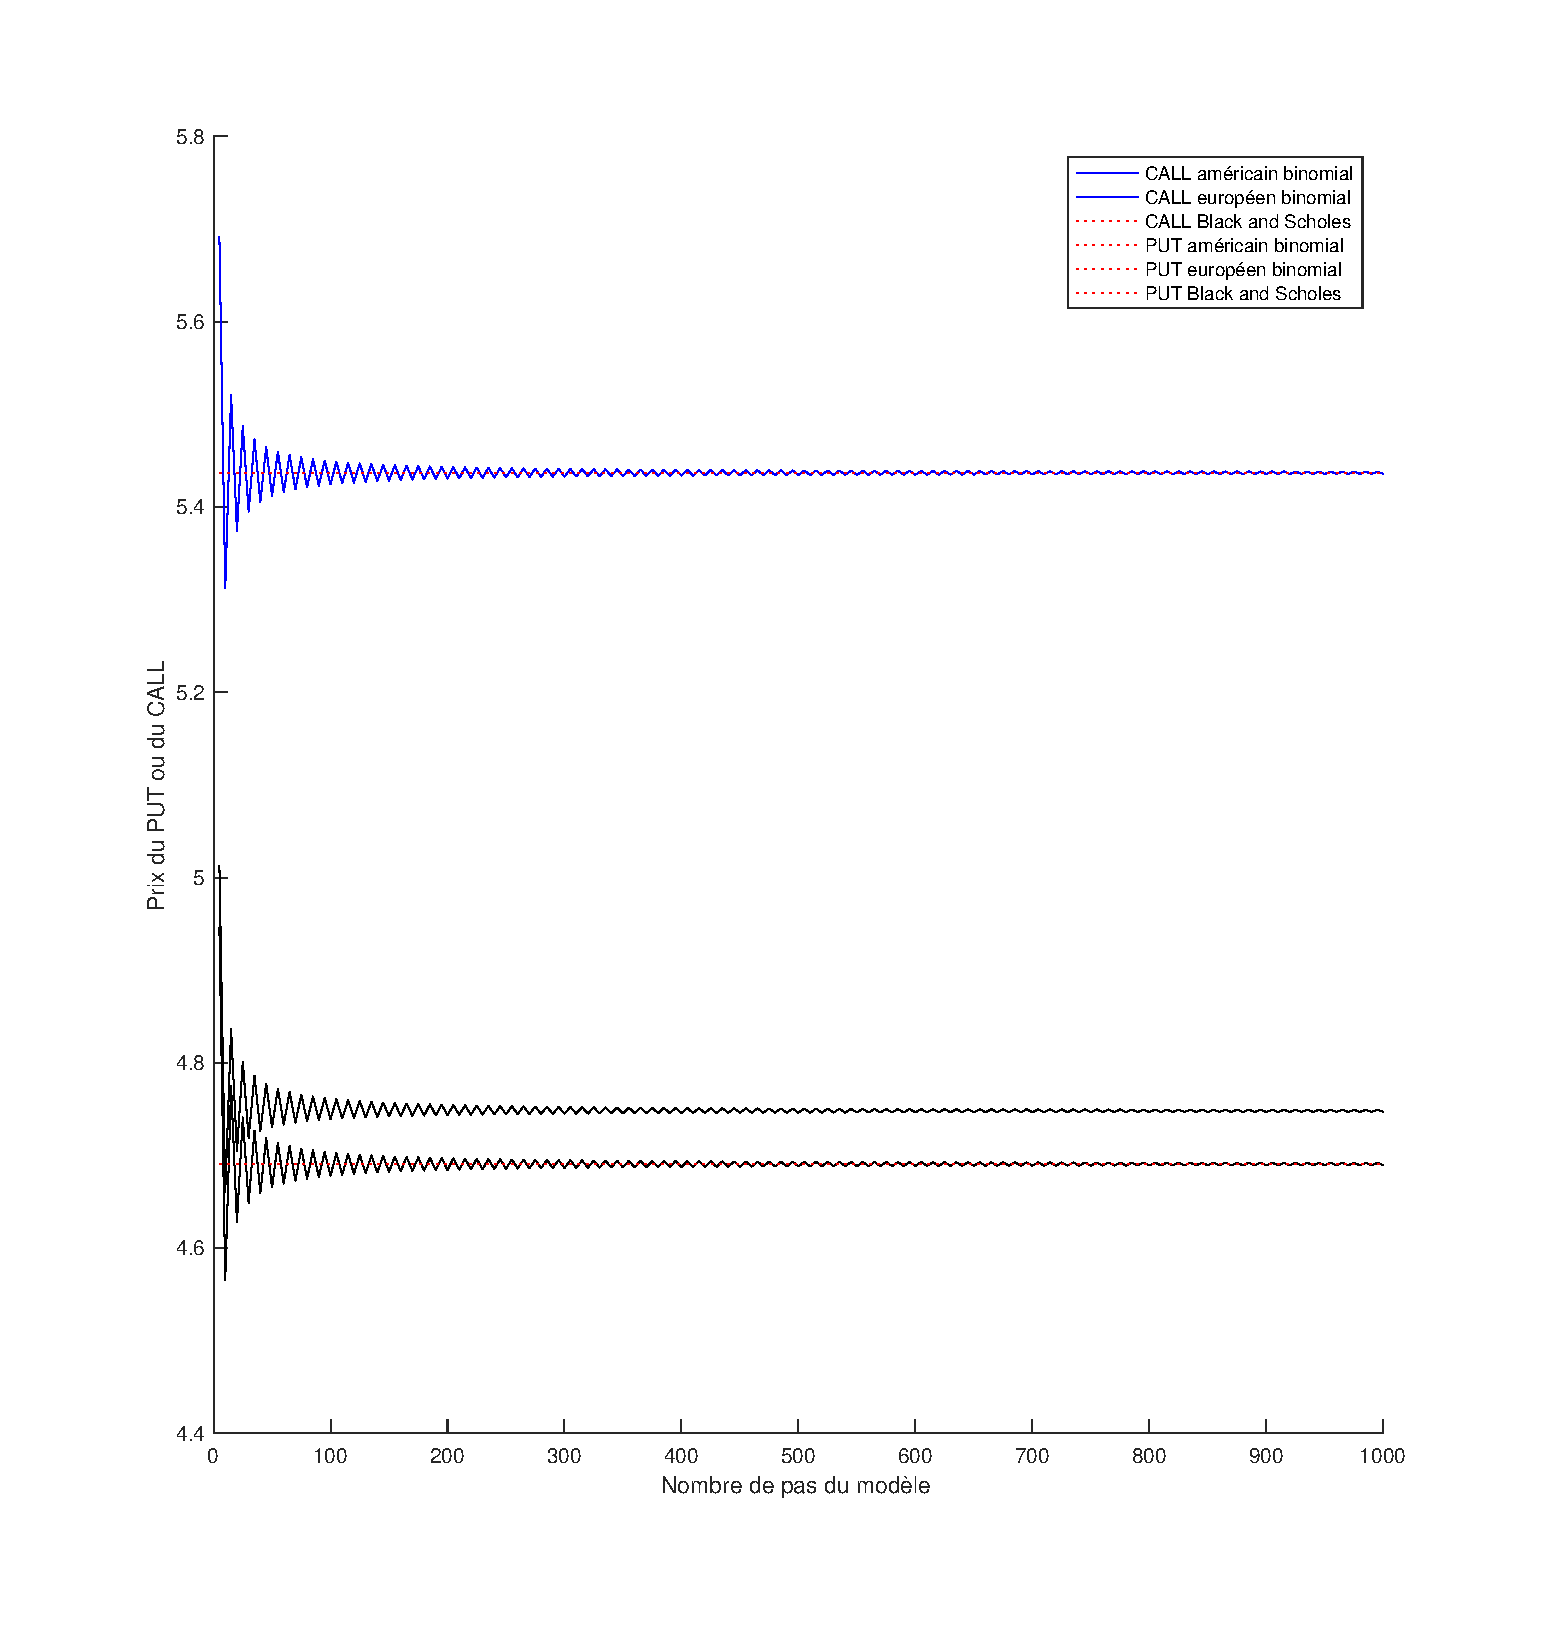
\includegraphics[scale=0.6]{./img/CALL_A_E-PUT_A_E-BS.eps}
\caption{Variation de l'ensemble des options en fonction du nombre de pas}
\label{fig:evol_mb}
\end{figure}

On observe donc avec les graphiques ce que l'on a demontré au début de la section. Le prix d’un put américain est plus éleve que celui d'un put européen. Ce qui est lié au degré de liberté supplémentaire : elles peuvent-être exercées à n’importe quel moment. Le CALL lui est égal dans les 2 cas comme démontré antérieurement.

\subsection{Frontiere d'exercice d'une option americaine} % (fold)
\label{sub:frontiere_d_exercice_d_une_option_americaine}

On calcule ensuite à l'aide de la fonction Listing~\ref{listing:12} du code \textsc{arbre.py}, la frontiere d'exercice d'un PUT. Il est inutile de calculer celles d'un CALL car comme on l'a vu avant il n'est jamais exercé avant la date d'échéance, on a cependant implémenté une option pour le vérifier (elle donne évidemment \textsc{[]}).

\begin{figure}[H]
\centering
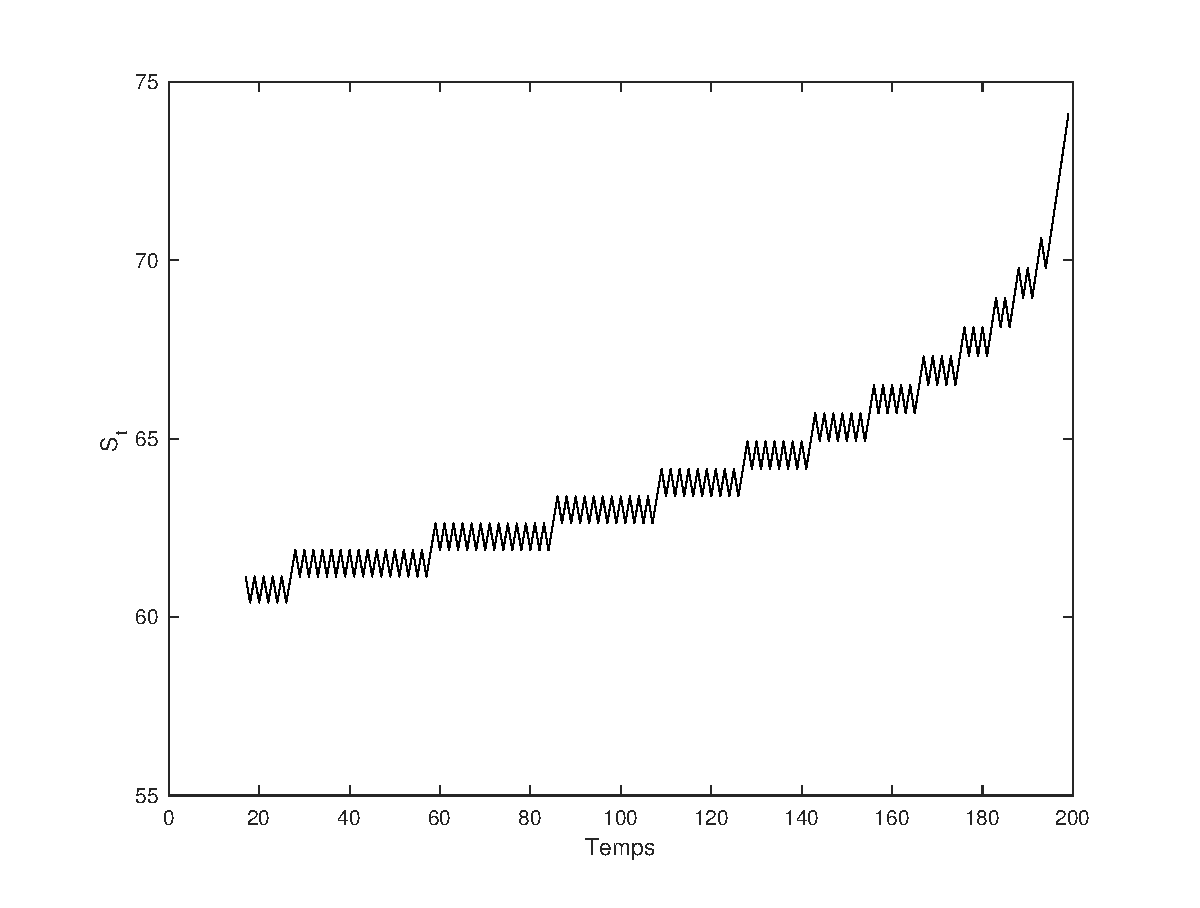
\includegraphics[scale=0.5]{./img/FRONTIERE_PUT.eps}
\caption{Frontiere d'exercice d'un put pour un nombre de pas $n=200$}
\label{fig:front_200}
\end{figure}

\begin{figure}[H]
\centering
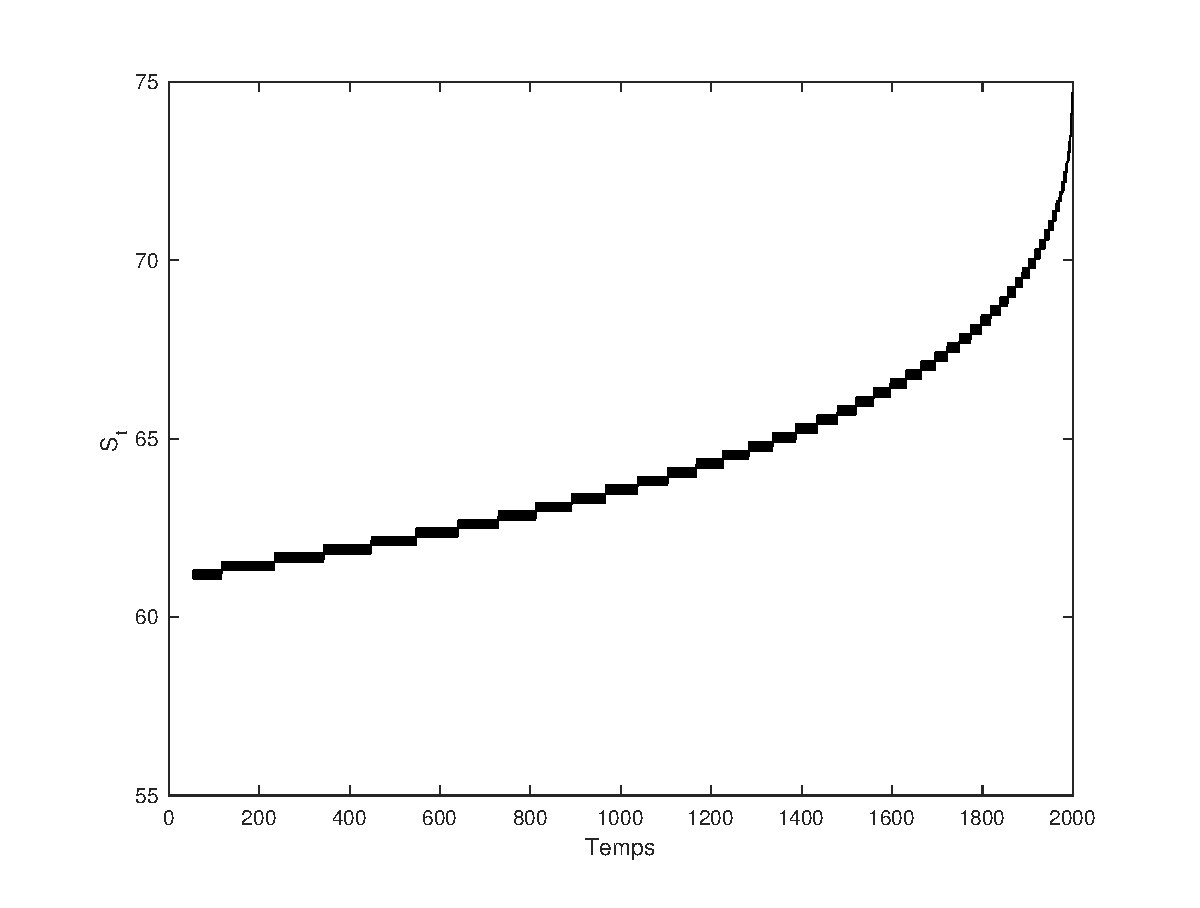
\includegraphics[scale=0.5]{./img/FRONTIERE_PUT_2000.eps}
\caption{Frontiere d'exercice d'un put pour un nombre de pas $n=2000$}
\label{fig:front_2000}
\end{figure}

% subsection frontiere_d_exercice_d_une_option_americaine (end)

% section question_3 (end)